\documentclass[]{beamer}
\usepackage{pgfpages}
\usepackage[utf8]{inputenc}
\usepackage[italian]{babel}
\usepackage{setspace}
\usepackage{color}
\usepackage{xcolor}
\usepackage{listings}
\usepackage{caption}
\usepackage{float}
\usepackage{hyperref} %for links in the table of contents
\hypersetup{hidelinks}
%color of code listings
\DeclareCaptionFont{white}{\color{white}}
\DeclareCaptionFormat{listing}{\colorbox{gray}{\parbox{\textwidth}{#1#2#3}}}
\captionsetup[lstlisting]{format=listing,labelfont=white,textfont=white}
%theme of slides
\usetheme{CambridgeUS}
%
\pgfdeclareimage[height=1cm]{logoUnipd}{img/unipd}
\pgfdeclareimage[height=2cm]{logoDei}{img/dei}
\logo{\pgfuseimage{logoUnipd}}
 \titlegraphic{\pgfuseimage{logoDei}}

\title[Note di credito]{Sviluppo della gestione delle note di credito in un
programma di fatturazione}
\author[Davide Fontana]{Laureando: Davide Fontana \\Relatore: Ch.mo Prof.\ Carlo Ferrari }
\date[Data pié di pagina]{Data \\ Anno accademico 2015/2016}
\institute[DEI Unipd]{Corso di Laurea in Ingegneria Informatica\\ Department of Information Engineering}

\begin{document}

    \frame{\titlepage}

    \begin{frame}
        \frametitle{Attività svolte}
        \begin{enumerate}
            \item Corso di formazione.
            \item Attività di bug-fixing.
            \item Programma per la gestione delle note di credito.
        \end{enumerate}
    \end{frame}

    \begin{frame}
        \frametitle{Azienda Ospitante}
        \begin{figure}[H]
            \centering
            \includegraphics[scale=0.4]{img/consoft}\label{logo:consoft}
        \end{figure}
    \end{frame}

    \begin{frame}
        \begin{center}
            \Huge Corso di formazione.
        \end{center}
    \end{frame}

    \begin{frame}
        \frametitle{Tecnologie imparate}
        \begin{itemize}
            \item Hibernate
            \item Spring
        \end{itemize}
    \end{frame}

    \begin{frame}
        \frametitle{Hibernate}
        Vantaggi:
        \begin{itemize}
            \item Tutta la gestione della connessione al database viene gestita 
                dal framework.
            \item Il reperimento dati viene fatto chiamando funzioni di Hibernate e 
                non più scrivendo query. 
            \item Tutto quello che viene restituito dalle funzioni di Hibernate sono
                oggetti Java.
        \end{itemize}
    \end{frame}

    \begin{frame}
        \frametitle{Spring}
        \begin{figure}[H]
            \centering
            \includegraphics[scale=0.2]{img/spring_logo}\label{spring:logo}
        \end{figure}
    \end{frame}

    \begin{frame}
        \frametitle{Spring MVC}
        \begin{figure}[H]
            \centering
            \includegraphics[scale=0.3]{img/spring_mvc_structure}\label{spring:diagram}
        \end{figure}
    \end{frame}

    \begin{frame}
       \frametitle{Esempio Spring MVC\@: Controller}
       \lstinputlisting[basicstyle=\tiny]{code/controller-example.java}
    \end{frame}

    \begin{frame}
       \frametitle{Esempio Spring MVC\@: View}
       \lstinputlisting[basicstyle=\tiny, firstline=16, lastline=37]{code/example-page.jsp}
    \end{frame}

    \begin{frame}
       \frametitle{Esempio Spring MVC\@: Pagina finale}
       \begin{figure}[H]
           \centering
           \includegraphics[scale=0.3]{img/spring_view_result}\label{spring:final_view}
       \end{figure}
    \end{frame}

    \begin{frame}
        \begin{center}
            \Huge Il programma di fatturazione.
        \end{center}
    \end{frame}

    \begin{frame}
        \frametitle{Lista dei package}
        \begin{itemize}
        \item \texttt{it.consoft.fatturazione.controller}
        \item \texttt{it.consoft.fatturazione.form}    
        \item \texttt{it.consoft.fatturazione.bean}
        \item \texttt{it.consoft.fatturazione.utils}
        \item \texttt{it.consoft.fatturazione.dao}
        \item \texttt{it.consoft.fatturazione.service}
        \end{itemize}
    \end{frame}

    \begin{frame}
        \frametitle{Data Access Object Pattern}
        \begin{figure}[H]
             \centering
             \includegraphics[scale=.4]{img/data-access-pattern-class-diagram}\label{pattern:dao}
         \end{figure}
    \end{frame}

    \begin{frame}
        \begin{center}
            \Huge Progetto delle note di credito    
        \end{center}
    \end{frame}

    \begin{frame}
        \frametitle{Analisi dei requisiti}
        Utilizzo della nota di credito:
        \begin{itemize}
            \item Correttiva parziale.
            \item Annullamento di una fattura.
        \end{itemize}
    \end{frame}

    \begin{frame}
        \frametitle{Database: Schema concettuale}
        \begin{figure}[H]
            \centering
            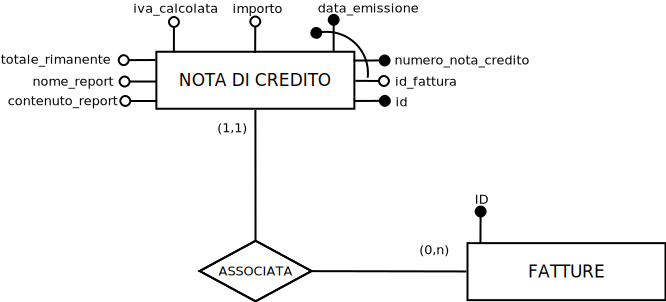
\includegraphics[scale=0.3]{img/schema_concettuale}\label{schema:concettuale}
        \end{figure}
    \end{frame}

    \begin{frame}
        \frametitle{Database: Schema logico}
        \begin{figure}[H]
            \centering
            \includegraphics[scale=0.3]{img/schema_logico}\label{schema:logico}
        \end{figure}
    \end{frame}

    \begin{frame}
        \frametitle{Database: Codice SQL}
        \lstinputlisting[basicstyle=\tiny]{code/tabella.sql}
    \end{frame}

    \begin{frame}
        \begin{center}
            \Huge Implementazione 
        \end{center}
    \end{frame}

\end{document}

